\documentclass{standalone}

\usepackage{pgfplots}

\pgfplotsset{compat=1.17}

\begin{document}
    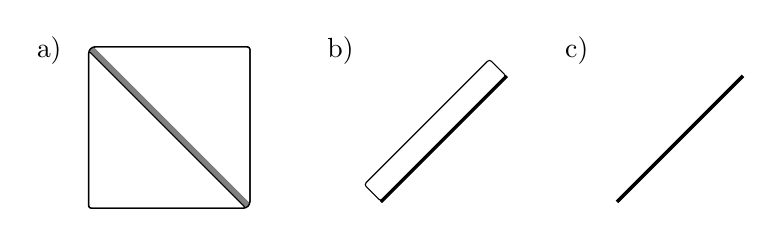
\begin{tikzpicture}
        \begin{scope}
            \node at (-0.5, 2) {a)};
            \coordinate (prism1 a) at (0, 0);
            \coordinate (prism1 b) at (2, 0);
            \coordinate (prism1 c) at (0, 2);
            \draw (prism1 b) ++(0.05, 0.05) coordinate (prism2 a);
            \draw (prism1 c) ++(0.05, 0.05) coordinate (prism2 c);
            \draw[rounded corners=1] (prism2 a) -- ++(0, 2) coordinate (prism2 b) -- (prism2 c) -- cycle;
            \filldraw[gray, rounded corners=1] (prism1 b) -- (prism2 a) -- (prism2 c) -- (prism1 c) -- cycle;
            \draw[rounded corners=1] (prism1 a) -- (prism1 b) -- (prism1 c) -- cycle;
            \draw[line width=0.5, rounded corners=1] (prism1 a) -- (prism1 b) -- (prism2 a) -- (prism2 b) -- (prism2 c) -- (prism1 c) -- cycle;
        \end{scope}

        \node at (3.2, 2) {b)};
        \begin{scope}[xshift=3.5cm, yshift=0.3cm, rotate=-45]
            \draw[rounded corners=1] (0, 0) rectangle (0.3, 2.25);
            \filldraw[black] (0.29, 0) rectangle (0.32, 2.25);
        \end{scope}

        \node at (6.2, 2) {c)};
        \begin{scope}[xshift=6.5cm, yshift=0.3cm, rotate=-45]
            \filldraw[black] (0.29, 0) rectangle (0.32, 2.25);
        \end{scope}
    \end{tikzpicture}
\end{document}
